% ======================================================================
\chapter{Training and testing: from simulators to real networks}
\label{ch:training}
% ======================================================================

This chapter answers \RQ{2}: how RL congestion controllers are trained and tested, and whether they still work on networks they did not see. We first define the \emph{evaluation ladder} from simulation to production (\cref{sec:ladder}) and measure where the corpus stands on it (\cref{sec:where}). We then examine evaluation practices (\cref{sec:practices}) and the evidence on generalization (\cref{sec:generalization}). A small reproducible case study isolates the effect of the training distribution (\cref{sec:case-study}), and we close with recommendations (\cref{sec:recommendations}).

% ----------------------------------------------------------------------
\section{The evaluation ladder}
\label{sec:ladder}

We distinguish four rungs, ordered by how much of the real system they include.

\begin{enumerate}
  \item \textbf{Simulation} models both the network and the endpoints. Packet-level discrete-event simulators (ns-2, ns-3, OMNeT++/INET, ndnSIM) model queues and protocols in detail. Custom simulators, often fluid or packet-level Python models such as Aurora's, trade fidelity for speed. Gym bridges connect RL libraries to them: ns3-gym~\cite{gawlowicz2019ns3gym}, Park~\cite{mao2019park}, RayNet for OMNeT++~\cite{giacomoni2024raynet}, and Gymir5G for 4G/5G~\cite{smirnov2024gymir5g}. Simulation is fast, controllable and repeatable. However, it leaves out the operating system's network stack: timers, pacing, segmentation offload, ACK aggregation and recovery heuristics.
  \item \textbf{Emulation} runs real protocol stacks and applications over links whose behavior is imposed in software. Mininet~\cite{lantz2010mininet} builds virtual topologies, and Mahimahi~\cite{netravali2015mahimahi} replays recorded cellular or wired link traces. NetEm adds delay, loss and jitter. Pantheon's emulators are calibrated so that their results match real Internet paths~\cite{yan2018pantheon}, and iBox learns path models from traces~\cite{ashok2020ibox,ashok2022data}. Emulation exercises the real controller code, but the link is still a model.
  \item \textbf{Shared and hardware testbeds} put real stacks on real links under controlled conditions. Examples are Pantheon's nodes on wired, cellular (LTE/UMTS) and Wi-Fi networks in ten countries~\cite{yan2018pantheon}, OpenNetLab's distributed nodes for real-time media~\cite{eo2022opennetlab}, 5G, Wi-Fi and satellite testbeds, and NIC or switch labs in data centers.
  \item \textbf{Real networks and production} expose the controller to real paths and traffic: experiments between cloud regions, A/B tests on a fraction of users, or full deployment.
\end{enumerate}

\noindent In our coding, rung~3 counts as ``real network'' when the links are physical, and as ``emulation'' when they are emulated. \Cref{tab:real} in \cref{app:tables} lists what ``real'' means for every study at that level.

\paragraph{A note on Wireshark.} Our project proposal described the path ``from simulators (Wireshark) to shared testbeds (Pantheon) and real networks''. That was a mistake that we correct here. Wireshark is a \emph{packet analyzer}: it captures and decodes traffic on a real or emulated interface. It does not generate traffic or model a network, so it is not a simulator. Packet capture is useful on every rung, for example to inspect a testbed trace, to validate an emulator against a real path, or to debug a controller's behavior in a kernel. The simulators in this literature are ns-2, ns-3, OMNeT++ and custom models, and the emulators are Mininet, Mahimahi and NetEm.

% ----------------------------------------------------------------------
\section{Where the corpus stands}
\label{sec:where}

\Cref{fig:evaluation} shows the highest evaluation level reached by the \nEmpiricalN{} empirical studies (all included studies except formal analyses). \nLevelSimulation{} studies (\nPctLevelSimulation\%) stop at simulation, \nLevelEmulation{} (\nPctLevelEmulation\%) at emulation, and \nLevelRealnetwork{} (\nPctLevelRealnetwork\%) reach a real network. The remaining \nLevelNotreported{} (\nPctLevelNotreported\%) do not report their environment in the material we could access. These are mostly studies coded from abstracts, which typically say ``extensive experiments'' without saying where. Among the \nKnownLevelN{} studies whose level is known, \nPctSimOnlyOfKnown\% are simulation-only and \nPctRealOfKnown\% reach a real network. In the subset coded from full texts, which is more complete but skewed toward prominent venues, \nPctRealOfFT\% reach a real network.

\begin{figure}[t]
\centering
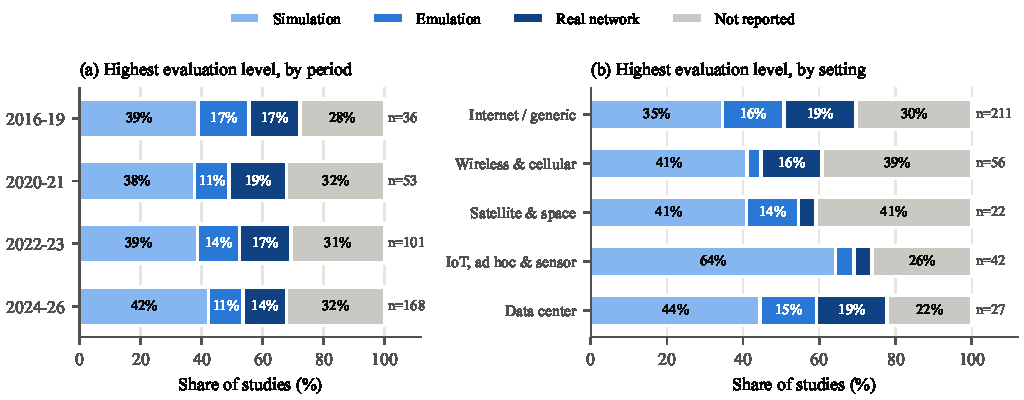
\includegraphics[width=\linewidth]{figures/fig_evaluation.pdf}
\caption{Highest evaluation level of the \nEmpiricalN{} empirical studies, (a)~by period of first report and (b)~by setting. Segments without a label are below 9\%. ``Not reported'' means the level could not be determined from the material we could access.}
\label{fig:evaluation}
\end{figure}

\paragraph{Trend over time.} Evaluations have become less realistic as the field has grown, even though tools such as Pantheon, Mahimahi and OpenNetLab have become standard (\cref{fig:evaluation}a). Studies first reported in 2020--21 reached a real network in \nPeriodBReal\% of cases and those from 2022--23 in \nPeriodCReal\%. For 2024--26 the share is \nPeriodDReal\%, while the simulation-only share rose from \nPeriodBSim\% to \nPeriodDSim\%. Simulation-only studies account for the largest part of the field's recent growth, and they dominate the IoT and wireless settings (\cref{fig:evaluation}b). By setting, Internet studies are the most realistic, and IoT, ad hoc and sensor studies the least. Two thirds of the latter are simulation-only.

\finding{As the field grew, the share of studies that reach a real network fell from \nPeriodBReal\% (2020--21) to \nPeriodDReal\% (2024--26). Only \nPctGen\% of design studies test outside their training distribution, and only \nPctCodeDesign\% release code.}

\paragraph{What ``real'' means.} Even the \nLevelRealnetwork{} real-network studies vary widely (\cref{tab:real}). Most run between cloud or testbed hosts over Internet paths. Deployment in production systems or user-facing tests is rare; \cref{tab:deployments} lists the nine studies that report it. Examples are OnRL's month-long evaluation on a live-streaming platform~\cite{zhang2020onrl}, Loki in a commercial RTC service~\cite{zhang2021loki}, ACC in production data centers~\cite{yan2021acc}, TCP-RL at a search engine~\cite{nie2019tcprl}, and Floo in a mobile web service~\cite{zhang2023floo}.

\paragraph{Where agents are trained.} The training environment is reported by \nTrainReported{} of the \nDesignN{} design studies. Simulators dominate (\nTrainSim, of which \nTrainNsThree{} use ns-3), followed by emulators (\nTrainEmu), testbeds (\nTrainTestbed), real networks (\nTrainReal) and logged datasets (\nTrainData). Training in simulation is reasonable, since exploration on a real network is slow and risky. However, it makes testing outside the simulator essential, and that testing is what the corpus most often lacks.

% ----------------------------------------------------------------------
\section{Evaluation practices}
\label{sec:practices}

\Cref{tab:practices} reports how often design studies follow the evaluation practices we coded, across all \nDesignN{} design studies and across the \nDesignFT{} whose full text we coded. Because abstracts omit details, the whole-corpus figures are lower bounds; the full-text figures come from a sample that over-represents prominent venues and are better read as upper bounds.

\begin{table}[t]
\centering
\caption{Evaluation practices of design studies: all \nDesignN{} design studies and the \nDesignFT{} coded from full texts. ``Tested on conditions outside the training range'' requires an explicit train/test split along at least one network parameter.}
\label{tab:practices}
\small
\begin{tabular}{@{}lrrrr@{}}
\toprule
 & \multicolumn{2}{c}{All design studies} & \multicolumn{2}{c}{Full-text subset} \\
\cmidrule(lr){2-3}\cmidrule(l){4-5}
Practice & $n$ & \% of 266 & $n$ & \% of 64 \\
\midrule
Code or artifact released & 22 & 8 & 17 & 27 \\
Tested on conditions outside the training range & 30 & 11 & 13 & 20 \\
Fairness or TCP-friendliness evaluated & 54 & 20 & 24 & 38 \\
Evaluated in emulation or on a real network & 75 & 28 & 27 & 42 \\
Evaluated on a real network & 43 & 16 & 13 & 20 \\
Evaluation environment not reported & 86 & 32 & 4 & 6 \\
\bottomrule
\end{tabular}

\end{table}

\paragraph{Code and artifacts.} Only \nPracCodeOrArtifactReleasedAll{} design studies (\nPctCodeDesign\%) release code, and even in the full-text subset only about a quarter do. In the full texts we read, comparisons with learned baselines therefore tend to involve the few controllers with public code (Aurora, Orca, Indigo, and the online-learning PCC Vivace), sometimes re-implemented. Newer learned designs are rarely compared with each other.

\paragraph{Generalization testing.} Only \nPracTestedOnConditionsOutsidAll{} design studies (\nPctGen\%) explicitly test on network conditions outside their training range. Many others evaluate on held-out traces or seeds from the \emph{same} distribution. That measures overfitting to individual traces but not robustness to distribution shift.

\paragraph{Fairness and friendliness.} Fairness is evaluated in \nPracFairnessOrTcpFriendlinesAll{} design studies (\nPctFair\%). In the full texts we read, most of these evaluations measure Jain's index among copies of the same controller rather than the \emph{harm} done to the deployed base~\cite{ware2019beyond}.

\paragraph{Practice scores.} Combining the five practices into the appraisal score of \cref{sec:appraisal} shows how rarely they occur together. The median design study satisfies only \nScoreMedian{} of the five (\nScoreMedianFT{} in the full-text subset). Of all design studies, \nScoreAtMostOne{} (\nPctScoreAtMostOne\%) satisfy at most one, and only \nScoreFourPlus{} satisfy four or more: \scoreExemplars. Of these, only Orca satisfies all five. These exemplars carry the most weight in this survey's conclusions.

\paragraph{Independent evaluations.} Four independent large-scale evaluations re-run many published learned controllers under common conditions. Abbasloo et al.\ propose general benchmarks that rank Internet controllers and find large room for improvement~\cite{abbasloo2023internet}. Giacomoni and Parisis evaluate public RL controllers reproducibly. They find that the controllers acquire bandwidth quickly and resist random loss, but cause excess loss, are unfair in almost all setups and lag when bandwidth or latency changes~\cite{giacomoni2024rlcc}. Mazilu et al.\ reach similar conclusions against CUBIC and BBRv3 and show that fairness terms in the reward do not generalize~\cite{mazilu2025learning}. CCLab attacks controllers with an RL adversary that perturbs inputs or the environment within bounds. It finds learned controllers (Orca, Canopy) generally \emph{more} robust than classic ones, and it shows that adversarial traces train more robust controllers~\cite{chen2026cclab}. Shared benchmarks have also emerged for real-time media, namely OpenNetLab, the MMSys'24 offline-RL challenge and ReCoCo's train/test trace split~\cite{eo2022opennetlab,khairy2024acm,markudova2026advancing}, along with automated assessment frameworks~\cite{pazhooheshy2025mahak} and a survey of congestion-control evaluation methodology in general~\cite{vielhaus2026evaluating}.

% ----------------------------------------------------------------------
\section{Evidence on generalization}
\label{sec:generalization}

\paragraph{Evidence of failure.} Learned controllers' sensitivity to their training assumptions was demonstrated before deep RL: Remy's machine-generated rules degraded when the network differed from the assumed model~\cite{sivaraman2014learnability}. Recent examples in the corpus are similar. Ghermezian et al.\ deployed an Aurora-style PPO controller, trained in simulation, on a 10\,Gbit/s wide-area path. It reached 0.5\% mean and 4.4\% peak utilization of the path, whereas CUBIC and BBR reached up to 9.9 and 9.7\,Gbit/s. The authors observe overshoot-and-collapse dynamics and call for scale-aware training~\cite{ghermezian2026ppo}. Iroko's agents overfit to the training topology~\cite{ruffy2018iroko}. Fang et al.\ document a gap between simulated and real reward for RTC~\cite{fang2019rtc}. A cellular ablation shows that higher training reward need not mean better network performance~\cite{naqvi2022ablation}. Valentine et al.\ show that a simulator's missing stack effects change an RL controller's behavior over LEO links~\cite{valentine2026emulation}. Adversarial studies find conditions, or competing flows, that degrade learned controllers severely~\cite{gilad2019robustifying,chen2025exploring}. One input-perturbation attack cuts throughput by about half and raises latency more than 36-fold~\cite{yang2022good}.

\paragraph{Evidence of success.} Aurora generalized to bandwidths more than 20$\times$ above its training range, though not to links where latency noise it never saw dominated the signal~\cite{jay2019aurora}. Tessler et al.'s RL-CC generalized to unseen data-center scenarios and later to live NICs~\cite{tessler2022rlcc,fuhrer2023nvidia}, and GraphCC handled unseen workloads and link failures~\cite{bernardez2024graphcc}. ReCoCo's best policies kept a 3--20\% QoE advantage on more than 3,000 unseen traces~\cite{markudova2026advancing}. The successes share a pattern: deliberately broad or adversarial training data, an architecture that limits the damage a bad decision can do, or both.

\paragraph{Methods for generalization.} \Cref{tab:gen-methods} organizes the methods proposed in the corpus into five families. The most widely used approach, hybridization, works mainly by bounding the damage a wrong decision can do rather than by making the policy itself generalize. We return to this distinction in \cref{ch:deployment}.

\begin{table}[t]
\centering
\caption{Methods proposed in the corpus to make learned controllers generalize, grouped by mechanism.}
\label{tab:gen-methods}
\small
\begin{tabularx}{\linewidth}{@{}L{3.3cm}YL{4.1cm}@{}}
\toprule
Family & Mechanism & Examples \\
\midrule
Shape the training distribution & Randomize link parameters; schedule environments by difficulty or by gap to a baseline; rebalance skewed traces; synthesize or adversarially generate traces & Aurora~\cite{jay2019aurora}, Genet~\cite{xia2022genet}, Plume~\cite{patel2023plume}, GenRL-CC~\cite{islam2026genrl}, CCLab~\cite{chen2026cclab} \\
Choose invariant inputs and rewards & Scale-free features; reward normalized by a capacity estimate; signals transformed to a common view across flows & Aurora~\cite{jay2019aurora}, Pacemaker-CC~\cite{chae2026pacemaker}, Jury~\cite{tian2025jury} \\
Adapt after deployment & Online learning in the field; transfer or fine-tuning; meta-RL with fast adaptation; specialized models per condition segment & OnRL~\cite{zhang2020onrl}, TRCC~\cite{zheng2023trcc}, MOCC~\cite{ma2022mocc}, meta-RL~\cite{mwaura2025adaptive,bai2025metacon,chen2025generalizable}, NMS~\cite{yao2025unified} \\
Learn from real data & Offline RL or imitation from logs of deployed controllers; training directly on real networks & Sage~\cite{yen2023sage}, MMSys'24~\cite{khairy2024acm}, Concerto~\cite{zhou2019concerto}, ARC~\cite{zhang2020reinforcement}, MARLIN~\cite{galliera2023marlin} \\
Bound the policy & Hybrid control with a classic algorithm; fallback under uncertainty; certified properties; verification to pick policies that generalize & Orca~\cite{abbasloo2020orca}, Spine~\cite{tian2024spine}, HAN~\cite{jia2026han}, Canopy~\cite{yang2024canopy}, Amir et al.~\cite{amir2024verifying} \\
\bottomrule
\end{tabularx}
\end{table}

% ----------------------------------------------------------------------
\section{Case study: how the training distribution shapes behavior outside it}
\label{sec:case-study}

Published studies rarely vary the training distribution while holding everything else fixed, so the corpus cannot say how much of a controller's out-of-distribution behavior is due to \emph{what it was trained on}. We therefore ran a small controlled experiment. Everything needed to reproduce it, including the environment, training, evaluation and figures, is in the replication package (\texttt{case\_study/}). Training takes about \nCsTrainMinutes{} minutes per seed on one CPU core.

\paragraph{Setup.} The environment is a fluid model of a single drop-tail bottleneck with Aurora's formulation~\cite{jay2019aurora}. The agent acts every 20\,ms monitor interval, and its feedback is delayed by one base RTT. It observes the latency gradient, latency ratio and sending ratio of the last ten intervals. Its action $a\in[-1,1]$ multiplies the rate by $(1+0.05a)$, or divides it by $(1-0.05a)$ when $a<0$, and its reward is utilization minus queueing delay in RTTs minus three times the loss rate. We trained PPO~\cite{schulman2017ppo} for \nCsSteps{} million steps with \nCsSeeds{} seeds under each of two training distributions:
\begin{itemize}
  \item \textbf{Narrow}: 1--5\,Mbit/s (similar to Aurora's training bandwidths), 40--60\,ms base RTT, buffers of 1--2 bandwidth-delay products (BDP), with no random loss, no RTT jitter and constant capacity.
  \item \textbf{Broad}: 1--100\,Mbit/s, 10--200\,ms, 0.2--5\,BDP, 0--3\% random loss, 0--10\,ms mean RTT jitter, and capacity that varies over time.
\end{itemize}
The baselines are a window-based, ACK-clocked Reno-like AIMD with slow start and a BBR-like controller with BBRv1's state machine and its in-flight cap of 2\,BDP. We evaluated every controller on 10-second flows, ramp-up included, while varying one factor at a time around a reference link inside the narrow range (3\,Mbit/s, 50\,ms, 1.5\,BDP).

\begin{figure}[t]
\centering
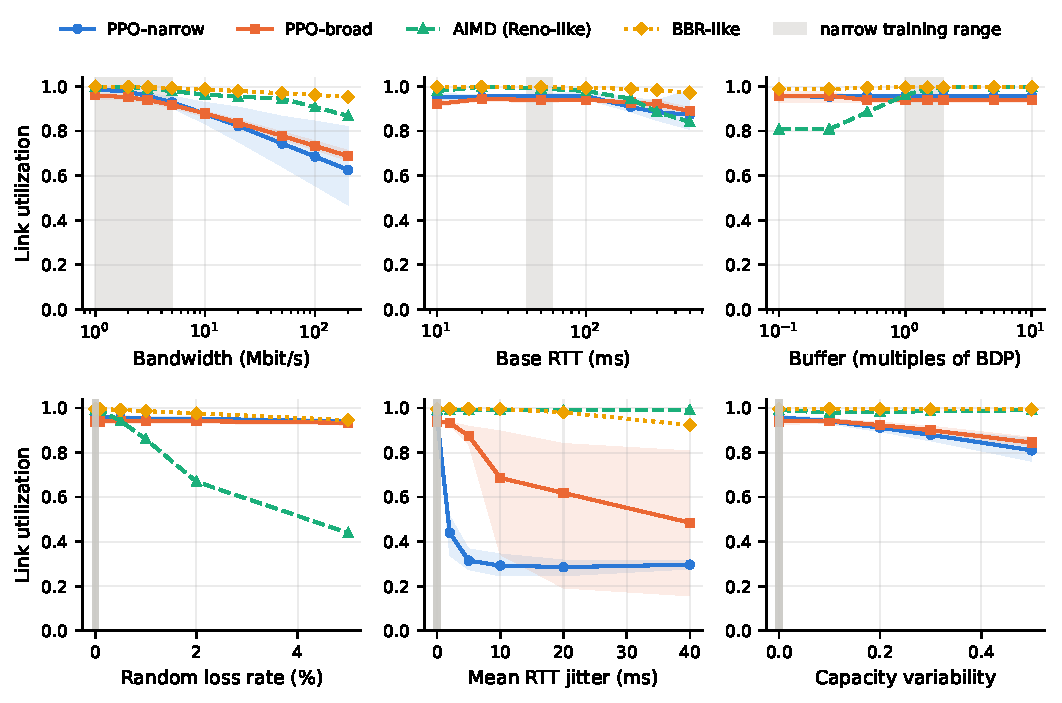
\includegraphics[width=\linewidth]{figures/case_study_util.pdf}
\caption{Case study: link utilization when one factor is varied around the reference link. Lines are means over the converged training seeds (as in \cref{tab:case}) and shaded bands span them; the one collapsed broad seed is excluded. The gray band or line marks the \emph{narrow} training range. The broad training range covers 1--100\,Mbit/s, 10--200\,ms, 0.2--5\,BDP, 0--3\% loss, 0--10\,ms jitter and capacity variability up to 0.3.}
\label{fig:case-util}
\end{figure}


\paragraph{Results.} \Cref{fig:case-util,tab:case} give the results (queueing delay is in \cref{fig:case-delay} in \cref{app:tables}).
\begin{enumerate}
  \item \textbf{In distribution.} Both learned policies reach at least \nCsBroadRefUtil\% utilization with queueing delay of \nCsNarrowRefQ{}--\nCsBroadRefQ{} RTT, against \nCsAimdRefQ{} RTT for AIMD. On its training distribution, the narrow policy scores best of all four controllers on the objective it was trained for (utilization minus queueing delay), slightly ahead of BBR-like, which has higher utilization but a larger queue.
  \item \textbf{RTT jitter.} With 10\,ms of mean RTT jitter, which is ordinary on Wi-Fi and cellular links, the narrow policy's utilization falls to \nCsNarrowJitterTenUtil\%. Its latency features read the noise as queue growth, and it backs off. AIMD, which ignores delay, and the BBR-like controller are unaffected (\nCsAimdJitterTenUtil\% and \nCsBbrJitterTenUtil\%). Aurora's authors observed the same failure mode: their policy performed poorly at 1\,ms latency because about 1\,ms of packet-processing noise, absent from training, dominated the latency signal~\cite{jay2019aurora}.
  \item \textbf{Broader training.} The broad policy, which saw up to 10\,ms of jitter, keeps \nCsBroadJitterTenUtil\% at 10\,ms but drops to \nCsBroadWorstUtil\% at 40\,ms, outside its range. In distribution it queues more (\nCsBroadRefQ{} vs.\ \nCsNarrowRefQ{} RTT). Training was also less reliable: one of \nCsSeeds{} broad seeds collapsed to \nCsCollapsedUtil\% utilization even on the reference link, whereas every narrow seed converged.
  \item \textbf{Random loss.} With 5\% random loss the PPO policies keep \nCsBroadLossFiveUtil--\nCsNarrowLossFiveUtil\% utilization, while AIMD falls to \nCsAimdLossFiveUtil\%. Their weakness is delay noise, so a test suite built around classic controllers' known weaknesses (random loss, shallow buffers) would rate the learned controller highly and miss how it fails.
  \item \textbf{High bandwidth.} At 200\,Mbit/s both PPO policies reach only \nCsNarrowBwTwoHundredUtil--\nCsBroadBwTwoHundredUtil\% utilization, against \nCsBbrBwTwoHundredUtil\% for BBR-like, even though the broad policy trained up to 100\,Mbit/s. Part of the gap is structural. An Aurora-style action changes the rate by at most 5\% per interval, so ramping up over two orders of magnitude takes seconds whatever the training data.
\end{enumerate}

\begin{table}[t]
\centering
\caption{Case study summary: mean over converged seeds and five flows per condition. ``Queue'' is the mean queueing delay in multiples of the base RTT. One of the \nCsSeeds{} broad training seeds collapsed (\nCsCollapsedUtil\% utilization even in distribution) and is excluded here; all \nCsSeeds{} narrow seeds converged.}
\label{tab:case}
\small
\begin{tabular}{@{}lrrrrrr@{}}
\toprule
 & \multicolumn{2}{c}{In distribution} & \multicolumn{4}{c}{Utilization (\%) under one shifted factor} \\
\cmidrule(lr){2-3}\cmidrule(l){4-7}
Controller & Util.\ (\%) & Queue (RTT) & 200\,Mbit/s & 5\% loss & 10\,ms jitter & Worst case \\
\midrule
PPO-narrow & 96 & 0.03 & 63 & 94 & 29 & 29 (20\,ms jitter) \\
PPO-broad & 94 & 0.09 & 69 & 93 & 69 & 49 (40\,ms jitter) \\
AIMD (Reno-like) & 99 & 0.72 & 87 & 44 & 99 & 44 (5\% loss) \\
BBR-like & 100 & 0.09 & 95 & 95 & 100 & 92 (40\,ms jitter) \\
\bottomrule
\end{tabular}

\end{table}

\finding{A learned controller's failure modes follow from its input features. Latency-based policies that perform well in distribution can collapse under ordinary delay noise that classic controllers ignore. In our experiment, broadening the training distribution helped only within the range it covered, and it reduced in-distribution quality and training stability.}

\paragraph{Caveats.} The model has one flow, a fluid queue and no competing traffic, and the policies are small. The experiment isolates the effect of the training distribution; it makes no claim about any published controller.

% ----------------------------------------------------------------------
\section{Recommendations for evaluating learned controllers}
\label{sec:recommendations}

From the corpus analysis and the case study we derive a reporting checklist (\cref{tab:checklist}). Several of its items echo advice from the evaluation literature~\cite{vielhaus2026evaluating,giacomoni2024rlcc}. We add a measurement of how often the corpus follows them.

\begin{table}[ht]
\centering
\caption{Checklist for evaluating RL congestion controllers. The rightmost column gives the share of design studies that already satisfy the item, where the corpus coding allows it to be measured.}
\label{tab:checklist}
\small
\begin{tabularx}{\linewidth}{@{}lYr@{}}
\toprule
\# & Item & Corpus \\
\midrule
C1 & State the training environment and the highest evaluation level (simulation, emulation, testbed, real, production) and name the tools. Do not call emulation ``real-world''. & \nPctPracEnvReported\% \\
C2 & Report the training distribution, and test at least one factor outside it. Include delay noise, capacity variation and competing traffic, not only random loss. & \nPctGen\% \\
C3 & Before claiming deployability, evaluate with real stacks: emulation at minimum, and trace-driven emulation for wireless and satellite links. & \nPctPracEmuReal\% \\
C4 & Compare with the deployed base (CUBIC, BBR) and at least one public learned controller, and measure harm to competing flows, not only Jain's index among copies. & \nPctFair\%$^{a}$ \\
C5 & Report results over several training seeds, including failed runs and their variance. & -- \\
C6 & Report inference cost, the decision interval, and where the model runs (kernel, user space, NIC, controller). & -- \\
C7 & Report worst-case and tail metrics alongside means. & -- \\
C8 & Release code, trained models and traces. & \nPctCodeDesign\% \\
\bottomrule
\multicolumn{3}{@{}l}{\footnotesize $^{a}$Share that evaluates fairness or friendliness in any form.}
\end{tabularx}
\end{table}
